\documentclass[11pt]{article}

\usepackage{common}
\usepackage{biblatex}
\usepackage{booktabs, hyperref}

\bibliography{ref}

\title{Practical 4: Reinforcement Learning}
\author{Emily Chen, Joanna Chung, Kevin Lee \\
Emails: emily-chen@, joannachung@, kevinlee01@college.harvard.edu}
\begin{document}


\maketitle{}

\section{Technical Approach}

Game playing is a classic reinforcement learning task. In class, we discussed Q-learning and SARSA as canonical algorithms for performing reinforcement learning. Although SARSA converges faster than Q-learning, it does not guarantee convergence to the optimal policy. Since we are learning the policy through offline simulations, fast convergence is not a primary concern. Thus, we decided to use Q-learning. We hoped that letting the procedure run for more iterations would enable it to converge to something closer to the optimal policy.

Q-learning is similar to policy evaluation for a Markov Decision Process. Because of the unknown gravity and randomness in the impulse from each jump, however,  the transition probabilities are unknown. Thus, it is useful to restate the Bellman equations to define a function $Q(s,a)$, from which the optimal policy can be determined. Then, $Q(s,a)$ can be iteratively estimated.

The primary challenge in this task comes from the intractability of fully tabulating $Q(s,a)$ for all possible discretizations of each state. The size of each component of the state space is:
\begin{align*}
    | \{\text{tree dist}\}| &= 600 \\ 
    | \{\text{tree top}\}| &\approx 200 \\ 
    | \{\text{tree bottom}\}| &\approx 200 \\ 
    | \{\text{monkey vel}\}| &\approx 120 \text{ (range of physically possible velocities)} \\ 
    | \{\text{monkey top}\}| &\approx 400 \\ 
    | \{\text{monkey bottom}\}| &\approx 400 \\ 
\end{align*}
Taking the product, there are approximately $4.6 \times 10^{14}$ possible states. Since the size of the action set is 2, the size of the support of $Q$ is $|S| \times |A| \approx 9.2 \times 10^{14}$. Thus, we cannot tabulate the Q-function in full detail. Instead, we must approximate the Q-function. We do so using two approaches: (linear) function approximation and quantization.

\subsection{Linear Function Approximation}

$Q(s,a)$ can be approximated as a linear combination of some features derived from the state space. In particular, we place weights $\theta_k$ on each of the 5 features plus the 4 feature interaction terms that define a state (described below) to calculate $Q(s,a)$ for each state-action pair and update them iteratively. The linear approximation is given as follows:
$$Q^a(s,a) = \theta^a_1 f_1 + \dots + \theta^a_n f_n$$
for each action $a$. In our case, there are 2 actions and $n=9$ total terms, so we have a total of 18 weights. The update rule for the weights is then:
$$\theta^a_k = \theta^a_k + \eta[r(s,a) + \gamma \max_{a'} Q^a(s',a') - Q^a(s,a)] \frac{dQ^a(s,a)}{d\theta^a_k}.$$ 
Here, $\eta$ is the learning rate and $\gamma$ is the discount factor. We construct our algorithm according to \cite{irodova2005reinforcement}.

From the features passed as the state from the swing monkey module, we constructed our own feature set. Given that the top of the monkey and bottom are a fixed distance apart, we used only the top position of the monkey. Likewise, we combined the top and bottom position of the tree. In addition to these two features, we used distance to tree, monkey velocity, and monkey acceleration (computed as the change in velocity from the previous state). After some experimentation, we noticed that the linear approximation algorithm did not provide for cross-dependencies between features, so we further added combinations of features: velocity x monkey height, monkey height x monkey velocity, distance to tree x tree height, monkey height x distance to tree.

\subsection{Quantization}

Alternatively, we can coarsen the state space, and then fully tabulate the Q-function on the coarsened space. Before doing so, we make some simplifications to the state space. Since the tree gap is constant, the positions of tree top and tree bot are redundant. Similarly, the monkey size is constant, so the positions of monkey top and monkey bot are redundant. Thus, we may drop monkey bot and tree bot from the information that encodes the state. 

Next, we divide each remaining component of the state space into the following bins:
\begin{itemize}
    \item Tree dist: $[0,100]$, $(100,200]$, $(200, 300]$, $(300, 450]$, $(450, \infty)$.
    \item Tree top: $[0,200], \ (200, 300], \ (300, \infty)$.
    \item Monkey top: $[0,50], \ (50, 100], \ (100, 150], \ (150, 200], \ (200, 250], \ (250, 300], \ (300, 350], \ (350, \infty)$.
    \item Monkey vel: $\ (-\infty, -20], \ (-20, 0], \ (0, 20], \ (20, 40], \ (40, \infty)$.
\end{itemize}
Note that the bins are not exactly evenly spaced. They are more finely spaced where we think more ``resolution'' would be appropriate. For example, it seems  worth the computational cost to have more bins when the monkey is closer to the tree than when it is far away. We also divided the monkey's position into finer bins because hitting the top or bottom of the screen is particularly bad, and this occurs purely as a function of the position.

This new state space has size $5 \times 3 \times 8 \times 5 = 600$, which is much smaller than $10^{14}$. Consequently, it is now feasible to fully tabulate $Q$ on this coarser support. 


\section{Results}
We ran both models for 1000 epochs. High scores were collected for various configurations of the learning rate $\eta$, discount factor $\gamma$, and $\epsilon$ value (decisions were made in an $\epsilon$-greedy manner).
\begin{table}[!h]
    \centering
    \begin{tabular}{c|c|c}
     \toprule
      & \textsc{Linear approx high score} & \textsc{Coarsened tabular high score}  \\
     \hline
     $\eta=0.5$, $\gamma=0.5$, $\epsilon=0.05$ & 15 & 7 \\
     $\eta=0.2$, $\gamma=0.5$, $\epsilon=0.05$ & 17 & 12 \\
     $\eta=0.1$, $\gamma=0.5$, $\epsilon=0.05$ & 15 & 16 \\
     $\eta=0.05$, $\gamma=0.5$, $\epsilon=0.05$ & 4 & 15 \\
     $\eta=0.2$, $\gamma=0.5$, $\epsilon=0.1$ & 14 & 9 \\
     $\eta=0.2$, $\gamma=0.85$, $\epsilon=0.05$ & 16 & 18 \\
     $\eta=0.2$, $\gamma=0.99$, $\epsilon=0.05$ & 5 & 12 \\
     \bottomrule
    \end{tabular}
\end{table}

Furthermore, we look at the scores over the epochs for one of the better configurations. The green on the left is for the linear approximation, and the blue on the right is for the tabular method.
\begin{center}
    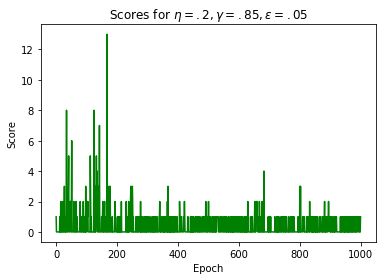
\includegraphics[scale=.5]{fun-scores.png}
    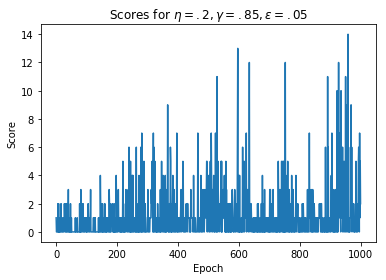
\includegraphics[scale=.5]{score-over-epochs.png}
\end{center}

Lastly, since the tabular method does not yet appear to have converged, we ran it for 10,000 epochs and recorded the scores.
\begin{center}
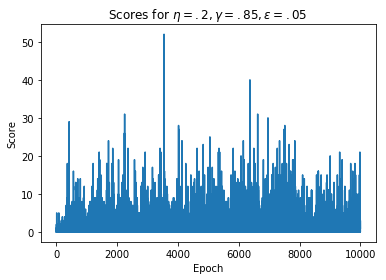
\includegraphics[scale =.5]{long-scores.png}
\end{center}

\section{Discussion}

Both methods performed similarly in terms of highest score achieved. The first model we tried, linear approximation, achieved a high score of 17, which is certainly better than the baseline score of 0 without learning. However, we believe that the linear nature of our model restricts the dependencies between the different states from being fully expressed, and may be the reason why we can't achieve scores that are much higher. Future experiments may include representing continuous state approximations using a different basis, such as radial or Fourier. Furthermore, the convergence behavior is odd, as initially the scores improve, but then they regress.

We wanted to perform better, so we created a tabular Q-value model, using bucketized states. After running for 10000 epochs, the tabular Q-learning algorithm appears to converge around epoch 8000, as the mean and variance appear to stabilize in the graph. Here the high score of 18 is comparable to the high score of 17 achieved by linear approximation. We were hoping for a significantly improved score, but we believe that the coarse nature of how we bucketized the state space, restricted by the size of the state space that we can run on our computers, may have lost too much resolution in the information of each feature. For example, the velocity difference between 10 and 20 may be significant in the monkey's performance, but in bucketizing these into one state, we lost valuable information and thus performance.

The first thing we would do if we had more time is tune hyperparameters more thoroughly. We would also explore different ways of adjusting the learning rate over time (which would hopefully improve convergence). Additionally, it would be interesting to consider better methods of function approximation, such as a neural nets. For the tabular case, further tuning of how to discretize/bucketize the state space and giving more resolution where it is shown to significantly impact performance may also help. This can be done by either manually testing different configurations, or perhaps employing parameters that might be learned as well. 

\printbibliography 

\end{document}